% Chapter Template

\chapter{Background} % Main chapter title

\label{Chapter3} % Change X to a consecutive number; for referencing this chapter elsewhere, use \ref{ChapterX}

\lhead{Chapter 3. \emph{Background}} % Change X to a consecutive number; this is for the header on each page - perhaps a shortened title

%----------------------------------------------------------------------------------------
%	SECTION 1
%----------------------------------------------------------------------------------------
In this chapter, we provide a brief description of the SWAN framework.
The first subsection will focus only on key features of SWAN, relevant to our work.
The second subsection will briefly describe few Beacon Frame Standards relevant for our research.

\section{SWAN}
The core functionality of SWAN is to act as a middleware between the phone applications and the hardware or software sensors.
We will further refer to the expression which is being passed to SWAN from application as SWANSong expression, or simply SWAN Song.
There are multiple types of SWANSong Expressions: \label{swan_song_expressions}
\begin{itemize}
 \item Value Expression - Retrieve values from sensors
 \item Tristate Expression - Perform evaluation on the values before sending them to applications
\end{itemize}

The application's interface with SWAN is always the same, the only component that varies is the SWANSong expression passed to SWAN.
SWANSong Expression (\hyperref[fig:SwanExpression]{Figure 3.1}) encapsulates all the information required by SWAN.
The main components of a SWANSong expression are:
\begin{itemize}
 \item Location - Tell SWAN were to evaluate the expression
 \item Sensor - Name of the SWAN Sensor
 \item Value Path - Identifies which value is requested
 \item Configuration - Web and local storage options
 \item Evaluation Options - Parameters for Evaluation Engine
\end{itemize}

Besides passing data to the application, SWAN also takes care of evaluation and storage. Relevant parameters are also embedded into the 
SWANSong expression.


\begin{figure}[htbp]
  \centering
    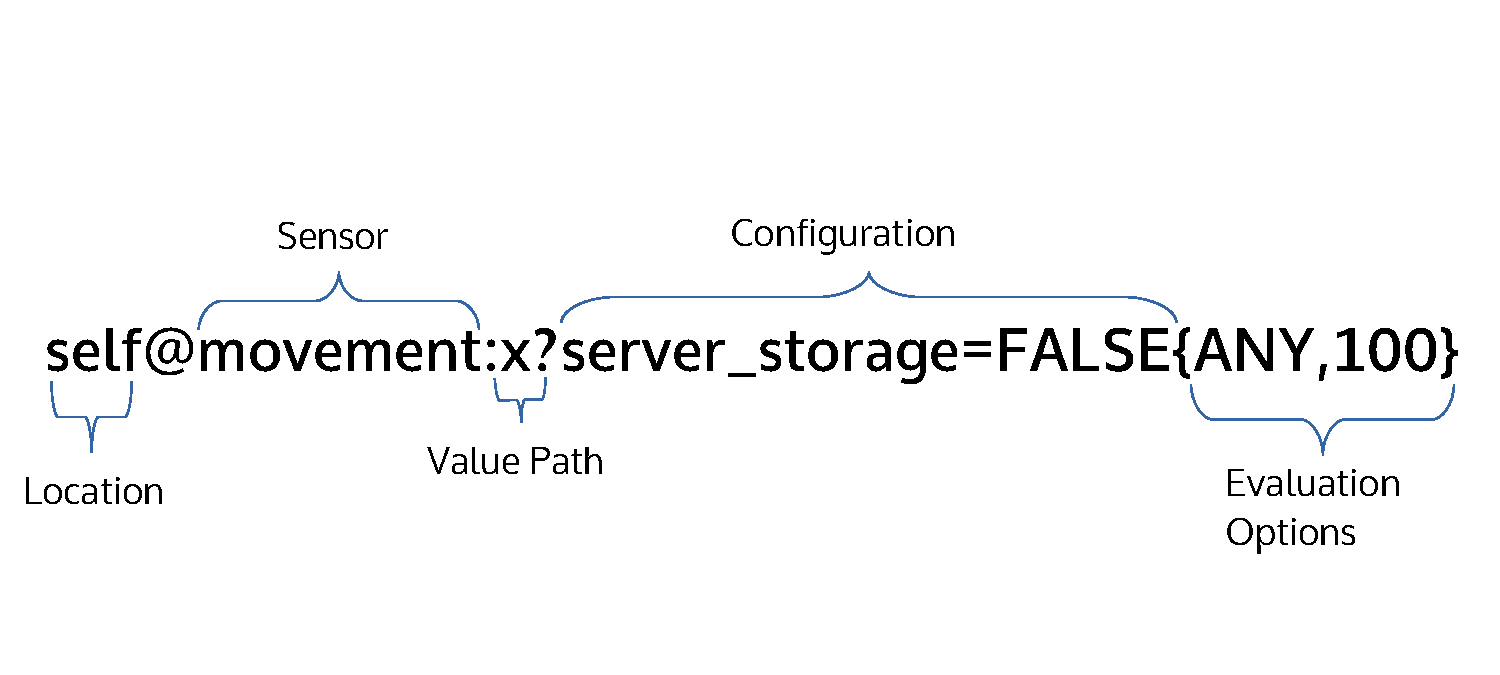
\includegraphics[scale=0.6]{Figures/swan_expr.pdf}
    \rule{35em}{0.5pt}
  \caption[Swan Expression]{Detailed SWAN expression}
  \label{fig:SwanExpression}
\end{figure}

As part of our research we will also apply changes on the SWAN Song Expression and the meaning of different parameters.

\section{Beacon Frame Standards}
With Bluetooth Low Energy devices market in its incipient stage, the Beacon  emitters suffer from high fragmentation.
To avoid the fragmentation of the Beacon Market, Google and Apple stepped in and proposed two standards for Beacon Frame Layout:

\begin{itemize}
 \item Apple iBeacon - simple beacon format, mostly used for proximity(distance measuring) applications
 \item Google Eddystone - complex standard, with 3 available frame formats:
 \begin{itemize}
  \item Eddystone UID - similar to iBeacon, broadcast unique ID
  \item EddystoneTLM - telemetry frame format, stores information about the beacon, such as temperature, battery level, number of packets sent
  \item Eddystone URL - frame layout which encodes a 17 bytes long URL in the frame
 \end{itemize}
\end{itemize}

The standards from above are industry recognized and widely implemented by various Beacon Manufacturers.
Unfortunately, even the Google Eddystone Format is not flexible enough and some companies need to come up with their own format to support extra functionality 
added to  their beacon products. We will also discuss the following frame formats which are proprietary to companies selling the test beacons, but they enable us to explore the
new way of using beacons:
\begin{itemize}
 \item AltBeacon Beacon Format - default beacon format present in the library used by SWAN for beacon scanning
 \item Estimote Nearable - Beacon Frame Format developed by Estimote\cite{estimote_company}, with accelerometer and movement data embedded into the format
\end{itemize}
